\documentclass{article}
\usepackage[utf8]{inputenc}
\usepackage{graphicx}
\usepackage{subcaption}
\usepackage{minted}

\title{CS544 -- MP 2}
\author{
	Zih-Siou Hung \\ zhung2@illinois.edu
	\and
	Patrick Cole \\ pacole2@illinois.edu
	\and
	Rajarshi Haldar \\ rhaldar2@illinois.edu
	\and
	Yuxuan Zhou \\ yuxuanz6@illinois.edu
}

\date{03/29/2019}

\begin{document}

\maketitle
\section{Objective}
Our homework2 is divided into the following parts: 
    
\begin{enumerate}
    \item Use the augmented Lagrangian method to find a surface that minimizes smoothness cost while interpolating points given below;Represent the surface as a height map on a 256 x 256 grid, representing the unit square.Represent the surface as a height map. Measure the smoothness as the norm of the gradient of the height map. The points to interpolate are: (0, 0, 1); (0, 1/2, 0); (0, 1, 1); (1/2, 0, 0); (1/2, 1/2, 1); (1/2, 1, 0); (1, 0, 1); (1, 1/2, 0); (1, 1, 1). Use a second order method to do the inner optimization.\label{qncq}
    \item Compare this solution with the solution obtained above by solving a linear system.\label{pr}
    \item Construct a surface of minimum area that interpolates these points and the line segments on the grid joining them  Use the augmented Lagrangian method.Plot the surface we
    get.\label{pr}
    \item Minimize the surface area of the interpolating surface that interpolates only the vertices. Plot the surface we get.\label{pr}
        
\end{enumerate}

We will analysis each part with our diagrams and code the following pages.

\newpage
\section{Analysis}
Within this analysis, we use the augmented Lagrangian method to find the minimum surface with the 9 given points and then we use the linear system to solve it compared with the augmented Lagrangian method. Next we construct a surface of minimum area that interpolates these points and the line segments on the grid. Last we minimize the surface area of the interpolating surface that interpolates only the vertices.
\subsection{part1 -- augmented  Lagrangian  method }



\begin{figure}[h]
      \centering
      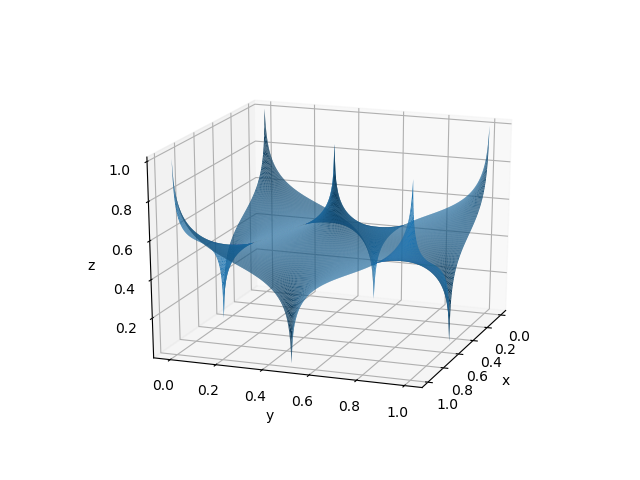
\includegraphics{figures/Figure_1.png}
      \caption{Augmented  Lagrangian  method surface}
\end{figure}


\subsection{part2 -- linear system  method }

\begin{figure}[h]
      \centering
      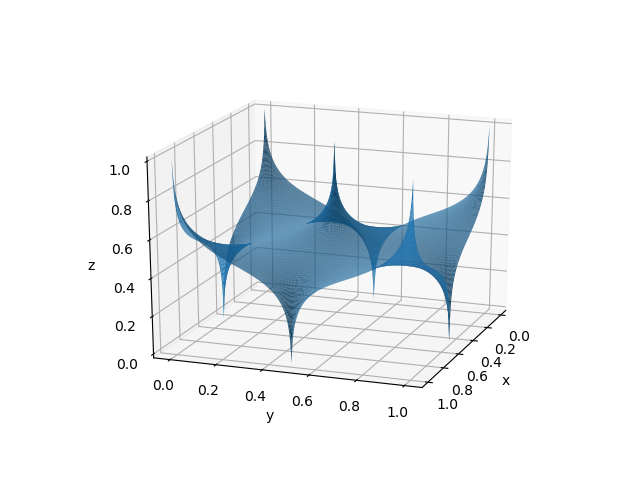
\includegraphics{figures/Figure_2.png}
      \caption{linear system method surface}
\end{figure}



\subsection{part3 -- interpolates these points and line segments}



\subsection{part4 -- interpolates only the vertices }



\section{Conclusion}
After all the studies and analysis completed, there are a few conclusions that can be made. 




\newpage
\section{Software Implementations}

Our source codes are provided in the following from part1 to part4. 

\subsection{part1.py}
\begin{minted}{python}
import numpy as np
import numpy.linalg as la
import matplotlib.pyplot as plt
from mpl_toolkits.mplot3d import Axes3D
from scipy.sparse import csr_matrix, eye
from scipy.optimize import minimize
from time import time

GRID_SIZE = 256

# Set up constraint
points = np.array([[0,0],[0,.5],[0,1],[.5,0],[.5,.5],[.5,1],[1,0],[1,.5],[1,1]])
cols = np.zeros(9)
for i in range(points.shape[0]):
    x,y = points[i]
    cols[i] = GRID_SIZE * np.floor((GRID_SIZE - 1) * x) + np.floor((GRID_SIZE - 1)  * y)

cols = cols.astype(np.int64)
rows = np.array([0,1,2,3,4,5,6,7,8])
data = np.array([1,1,1,1,1,1,1,1,1])

A = csr_matrix((data, (rows, cols)), shape=(len(cols), GRID_SIZE**2))
b = np.array([1,0,1,0,1,0,1,0,1])

# Set up Ay for cost func
Ay = -1 * eye(GRID_SIZE**2, GRID_SIZE**2, k=0)
Ay += eye(GRID_SIZE**2, GRID_SIZE**2, k=1)
# need to remove entries where it tries to compare
# h(x,255) to h(x+1,0)
for i in range(GRID_SIZE-1, GRID_SIZE**2, GRID_SIZE):
    Ay[i,i] = 0
    if (i+1 < GRID_SIZE**2):
        Ay[i,i+1] = 0

# Set up Ax for cost func
Ax = -1 * eye(GRID_SIZE**2, GRID_SIZE**2, k=0)
Ax += eye(GRID_SIZE**2, GRID_SIZE**2, k=GRID_SIZE)
# need to remove entries where it tries to compare
# h(255,y) to h(0,y+1)
lastValidEntry = GRID_SIZE**2 - GRID_SIZE
for i in range(lastValidEntry, GRID_SIZE**2):
    Ax[i,i] = 0

def f(x):
    return x.T @ Ax.T @ Ax @ x \
           + x.T @ Ay.T @ Ay @ x

def df(x):
    return 2 * Ax.T @ Ax @ x \
           + 2 * Ay.T @ Ay @ x

def g(x):
    return A @ x - b

def dg(x):
    return A

def ALM(x, lmbda, c):
    return f(x) - np.inner(lmbda,g(x)) + 0.5 * c * la.norm(g(x))**2

def dALM(x, lmbda, c):
    return df(x) - lmbda @ dg(x) + c * g(x) @ dg(x) 

# intial values for algorithm
c = 1.0
lmbda = np.ones(len(cols))
Vh = np.zeros(GRID_SIZE**2)

# Algorithm
start = time()
for i in range(5):
    print(f'Iteration {i+1}')
    res = minimize(ALM, Vh, args=(lmbda, c), method='L-BFGS-B', jac=dALM) #options={'maxiter': 50})
    Vh = res.x
    lmbda = lmbda - 0.5 * c * g(Vh)
    c = 2 * c
end = time()

print(f'Augmented Lagrangian took {end - start} seconds..')

# plot
h = Vh.reshape((GRID_SIZE,GRID_SIZE), order='F')

x = np.linspace(0,1,GRID_SIZE)
y = np.linspace(0,1,GRID_SIZE)
X, Y = np.meshgrid(x,y)

fig = plt.figure()
ax = plt.axes(projection='3d')
ax.set_xlabel('x')
ax.set_ylabel('y')
ax.set_zlabel('z')
ax.plot_surface(X, Y, h, rstride=1, cstride=1)
ax.view_init(20,20)

plt.show()
\end{minted}

\subsection{part2.py}
\begin{minted}{python}
import numpy as np
import numpy.linalg as la
import matplotlib.pyplot as plt
from mpl_toolkits.mplot3d import Axes3D
from scipy.sparse import csr_matrix, bmat, eye, coo_matrix
from scipy.sparse.linalg import lsqr

GRID_SIZE = 256

points = np.array([[0,0],[0,.5],[0,1],[.5,0],[.5,.5],[.5,1],[1,0],[1,.5],[1,1]])
cols = np.zeros(9)
for i in range(points.shape[0]):
    x,y = points[i]
    cols[i] = GRID_SIZE * np.floor((GRID_SIZE - 1) * x) + np.floor((GRID_SIZE - 1)  * y)

cols = cols.astype(np.int64)
rows = np.array([0,1,2,3,4,5,6,7,8])
data = np.array([1,1,1,1,1,1,1,1,1])

L = csr_matrix((data, (rows, cols)), shape=(len(cols), GRID_SIZE**2))
c = np.array([1,0,1,0,1,0,1,0,1])

# Set up Ay for cost func
Ay = -1 * eye(GRID_SIZE**2, GRID_SIZE**2, k=0)
Ay += eye(GRID_SIZE**2, GRID_SIZE**2, k=1)
# need to remove entries where it tries to compare
# h(x,255) to h(x+1,0)
for i in range(GRID_SIZE-1, GRID_SIZE**2, GRID_SIZE):
    Ay[i,i] = 0
    if (i+1 < GRID_SIZE**2):
        Ay[i,i+1] = 0

# Set up Ax for cost func
Ax = -1 * eye(GRID_SIZE**2, GRID_SIZE**2, k=0)
Ax += eye(GRID_SIZE**2, GRID_SIZE**2, k=GRID_SIZE)
# need to remove entries where it tries to compare
# h(255,y) to h(0,y+1)
lastValidEntry = GRID_SIZE**2 - GRID_SIZE
for i in range(lastValidEntry, GRID_SIZE**2):
    Ax[i,i] = 0

M = Ax.T @ Ax + Ay.T @ Ay
A = bmat([[M, L.T],[L, None]])
b = np.zeros((M.shape[0] + L.shape[0]))
b[M.shape[0]:] = c

H = lsqr(A, b)[0]
h = H[:M.shape[1]].reshape((GRID_SIZE,GRID_SIZE), order='F')

x = np.linspace(0,1,GRID_SIZE)
y = np.linspace(0,1,GRID_SIZE)
X, Y = np.meshgrid(x,y)

fig = plt.figure()
ax = plt.axes(projection='3d')
ax.set_xlabel('x')
ax.set_ylabel('y')
ax.set_zlabel('z')
ax.plot_surface(X, Y, h, rstride=1, cstride=1)
ax.view_init(20,20)

plt.show()
\end{minted}{python}

\subsection{part3.py}
\begin{minted}{python}
import numpy as np
import numpy.linalg as la
import matplotlib.pyplot as plt
from mpl_toolkits.mplot3d import Axes3D
from scipy.sparse import csr_matrix, eye
from scipy.optimize import minimize
from time import time

GRID_SIZE = 256

def getIndex(x, y):
    return GRID_SIZE * x + y

def interpolant(t, start, end, range_):
    return start + t * float(end - start) / range_
    

mid = GRID_SIZE // 2
cols = []
b = []

for y in range(GRID_SIZE):
    # first append is the first column
    # second append is the middle column
    # third append is the last column
    cols.append(getIndex(0,y))
    cols.append(getIndex(mid,y))
    cols.append(getIndex(GRID_SIZE - 1, y))
    if y <= mid:
        b.append(interpolant(y, 1, 0, mid))
        b.append(interpolant(y, 0, 1, mid))
        b.append(interpolant(y, 1, 0, mid))
    else:
        b.append(interpolant(y - mid, 0, 1, mid))
        b.append(interpolant(y - mid, 1, 0, mid))
        b.append(interpolant(y - mid, 0, 1, mid))

for x in range(GRID_SIZE):
    # first append is the first row
    # second append is the middle row
    # third append is the last row
    cols.append(getIndex(x,0))
    cols.append(getIndex(x,mid))
    cols.append(getIndex(x,GRID_SIZE - 1))
    if x <= mid:
        b.append(interpolant(x, 1, 0, mid))
        b.append(interpolant(x, 0, 1, mid))
        b.append(interpolant(x, 1, 0, mid))
    else:
        b.append(interpolant(x - mid, 0, 1, mid))
        b.append(interpolant(x - mid, 1, 0, mid))
        b.append(interpolant(x - mid, 0, 1, mid))

cols = np.array(cols)
rows = np.arange(len(cols))
data = np.ones(len(cols))

A = csr_matrix((data, (rows, cols)), shape=(len(cols), GRID_SIZE**2))
b = np.array(b)

# Set up Ay for cost func
Ay = -1 * eye(GRID_SIZE**2, GRID_SIZE**2, k=0)
Ay += eye(GRID_SIZE**2, GRID_SIZE**2, k=1)
# need to remove entries where it tries to compare
# h(x,255) to h(x+1,0)
for i in range(GRID_SIZE-1, GRID_SIZE**2, GRID_SIZE):
    Ay[i,i] = 0
    if (i+1 < GRID_SIZE**2):
        Ay[i,i+1] = 0

# Set up Ax for cost func
Ax = -1 * eye(GRID_SIZE**2, GRID_SIZE**2, k=0)
Ax += eye(GRID_SIZE**2, GRID_SIZE**2, k=GRID_SIZE)
# need to remove entries where it tries to compare
# h(255,y) to h(0,y+1)
lastValidEntry = GRID_SIZE**2 - GRID_SIZE
for i in range(lastValidEntry, GRID_SIZE**2):
    Ax[i,i] = 0

def f(x):
    return x.T @ Ax.T @ Ax @ x \
           + x.T @ Ay.T @ Ay @ x

def df(x):
    return 2 * Ax.T @ Ax @ x \
           + 2 * Ay.T @ Ay @ x

def g(x):
    return A @ x - b

def dg(x):
    return A

def ALM(x, lmbda, c):
    s = 0
    hx = Ax @ x
    hy = Ay @ x
    #'''
    h = x.reshape((GRID_SIZE, GRID_SIZE), order='F')
    areas = 0.5 * np.sqrt(1 + (h[:GRID_SIZE-1,1:] - h[:GRID_SIZE-1,:GRID_SIZE-1])**2 + (h[1:,:GRID_SIZE-1] - h[:GRID_SIZE-1,:GRID_SIZE-1])**2)
    areas+= 0.5 * np.sqrt(1 + (h[:GRID_SIZE-1,1:] - h[1:,1:])**2 + (h[1:,:GRID_SIZE-1] - h[1:,1:])**2)
    s = np.sum(areas)
    #'''
    '''
    for i in range(GRID_SIZE**2):
        for j in range(GRID_SIZE**2):
            s += np.sqrt(1 + hx[i] ** 2 + hy[i] ** 2)
    '''
    '''
    hx, hy = np.meshgrid(hx, hy, sparse=True)
    hx = hx ** 2
    hy = hy ** 2
    s = np.sum(np.sqrt(1 + hx + hy))
    '''
    #s = objective(hx, hy, GRID_SIZE)
    return s - np.inner(lmbda,g(x)) + 0.5 * c * la.norm(g(x))**2
    #return f(x) - np.inner(lmbda,g(x)) + 0.5 * c * la.norm(g(x))**2

def dALM(x, lmbda, c):
    return
    #return df(x) - lmbda @ dg(x) + c * g(x) @ dg(x) 

# intial values for algorithm
c = 1.0
lmbda = np.ones(len(cols))
Vh = np.zeros(GRID_SIZE**2)

# Algorithm
start = time()
for i in range(10):
    print(f'Iteration {i+1}')
    res = minimize(ALM, Vh, args=(lmbda, c), method='L-BFGS-B')#, jac=dALM, options={'maxiter': 50})
    Vh = res.x
    lmbda = lmbda - 0.5 * c * g(Vh)
    c = 2 * c
end = time()

print(f'Augmented Lagrangian took {end - start} seconds..')

# plot
h = Vh.reshape((GRID_SIZE,GRID_SIZE), order='F')

x = np.linspace(0,1,GRID_SIZE)
y = np.linspace(0,1,GRID_SIZE)
X, Y = np.meshgrid(x,y)

fig = plt.figure()
ax = plt.axes(projection='3d')
ax.set_xlabel('x')
ax.set_ylabel('y')
ax.set_zlabel('z')
ax.plot_surface(X, Y, h, rstride=1, cstride=1)
ax.view_init(20,20)

plt.show()
\end{minted}

\subsection{part4.py}
\begin{minted}{python}
import numpy as np
import numpy.linalg as la
import matplotlib.pyplot as plt
from mpl_toolkits.mplot3d import Axes3D
from scipy.sparse import csr_matrix, eye
from scipy.optimize import minimize
from time import time

GRID_SIZE = 256

# Set up constraint
points = np.array([[0,0],[0,.5],[0,1],[.5,0],[.5,.5],[.5,1],[1,0],[1,.5],[1,1]])
cols = np.zeros(9)
for i in range(points.shape[0]):
    x,y = points[i]
    cols[i] = GRID_SIZE * np.floor((GRID_SIZE - 1) * x) + np.floor((GRID_SIZE - 1)  * y)

cols = cols.astype(np.int64)
rows = np.array([0,1,2,3,4,5,6,7,8])
data = np.array([1,1,1,1,1,1,1,1,1])

A = csr_matrix((data, (rows, cols)), shape=(9, GRID_SIZE**2))
b = np.array([1,0,1,0,1,0,1,0,1])

# Set up Ay for cost func
Ay = -1 * eye(GRID_SIZE**2, GRID_SIZE**2, k=0)
Ay += eye(GRID_SIZE**2, GRID_SIZE**2, k=1)
# need to remove entries where it tries to compare
# h(x,255) to h(x+1,0)
for i in range(GRID_SIZE-1, GRID_SIZE**2, GRID_SIZE):
    Ay[i,i] = 0
    if (i+1 < GRID_SIZE**2):
        Ay[i,i+1] = 0

# Set up Ax for cost func
Ax = -1 * eye(GRID_SIZE**2, GRID_SIZE**2, k=0)
Ax += eye(GRID_SIZE**2, GRID_SIZE**2, k=GRID_SIZE)
# need to remove entries where it tries to compare
# h(255,y) to h(0,y+1)
lastValidEntry = GRID_SIZE**2 - GRID_SIZE
for i in range(lastValidEntry, GRID_SIZE**2):
    Ax[i,i] = 0

def f(x):
    return x.T @ Ax.T @ Ax @ x \
           + x.T @ Ay.T @ Ay @ x

def df(x):
    return 2 * Ax.T @ Ax @ x \
           + 2 * Ay.T @ Ay @ x

def g(x):
    return A @ x - b

def dg(x):
    return A

def ALM(x, lmbda, c):
    h = x.reshape((GRID_SIZE, GRID_SIZE), order='F')
    areas = 0.5 * np.sqrt(1 + (h[:GRID_SIZE-1,1:] - h[:GRID_SIZE-1,:GRID_SIZE-1])**2 + (h[1:,:GRID_SIZE-1] - h[:GRID_SIZE-1,:GRID_SIZE-1])**2)
    areas+= 0.5 * np.sqrt(1 + (h[:GRID_SIZE-1,1:] - h[1:,1:])**2 + (h[1:,:GRID_SIZE-1] - h[1:,1:])**2)
    s = np.sum(areas)
    return s - np.inner(lmbda,g(x)) + 0.5 * c * la.norm(g(x))**2
    #return f(x) - np.inner(lmbda,g(x)) + 0.5 * c * la.norm(g(x))**2

def dALM(x, lmbda, c):
    return df(x) - lmbda @ dg(x) + c * g(x) @ dg(x) 

# intial values for algorithm
c = 1.0
lmbda = np.ones(9)
Vh = np.zeros(GRID_SIZE**2)

# Algorithm
start = time()
for i in range(10):
    print(f'Iteration {i+1}')
    res = minimize(ALM, Vh, args=(lmbda, c), method='L-BFGS-B', options={'maxiter':50})#, jac=dALM, options={'maxiter': 50})
    Vh = res.x
    lmbda = lmbda - 0.5 * c * g(Vh)
    c = 2 * c
end = time()

print(f'Augmented Lagrangian took {end - start} seconds..')

# plot
h = Vh.reshape((GRID_SIZE,GRID_SIZE), order='F')

x = np.linspace(0,1,GRID_SIZE)
y = np.linspace(0,1,GRID_SIZE)
X, Y = np.meshgrid(x,y)

fig = plt.figure()
ax = plt.axes(projection='3d')
ax.set_xlabel('x')
ax.set_ylabel('y')
ax.set_zlabel('z')
ax.plot_surface(X, Y, h, rstride=1, cstride=1)
ax.view_init(20,20)

plt.show()
\end{minted}

\end{document}